\chapter*{Introduction}
The following work wants to explore the phases of the handshake between a human and a robot, reaching a consensus in the human-machine interaction. The handshake event can be divided in two steps: the approaching and handshaking. The consensus is a parameter that allow the human to evaluate a handshake mixing aspects like: duration of the event, dynamics, force exchanged etc.. 
The handshake is the most common human-human interaction and is extensively used worldwide in events like: greetings, introduction routine between human beings and agreements. 
This work focuses only on the latter handshake step, with the purpose of evaluating different ideas.
Many research teams all over the world are focused on the human-robot physical interaction, this makes opens the topic to an interesting scientific discussion.  


\chapter{The state of the Art}
Develop a robot capable of performing a smooth human-like handshake is still a highly interested topic in the scientific literature.
A natural handshake between two humans is a very complex task to replicate, this work just focuses on the interaction force between the artificial hand and the human hand.
The consensus is a complex task to encode inside a robot, the human will easily distinguish the event with respect to another human or to a robot. A human will take into consideration the skin feedbacks like: the temperature, the humidity and the softness. These are all characteristics that are still not embedded into the hardware available in the market. The aspect taken in consideration in this work is the grasping force, during the handshake. 
Robots, nowadays, are highly involved in industries where mostly they have to execute repetitive tasks. These kind of robots, when it comes to grasping objects, most of the times use grippers which are highly focused in the specific task. [insert a paper related to this study]

\cite{facialexpressions}
\cite{espen}
\cite{mirrorgame}
\cite{papageorgiou}

\chapter{The Idea}
The idea is to create a closed loop controller for the human-robot handshake event, using hardware as simple as the softhand produced for research purposes at Universit\'a degli studi di Pisa and augmenting it with four independent FSR sensors which uses an Arduino uno in order to communicate the data.
The FSR sensors are located on the robotic hand so there are no wearing device on the human in order to execute the experiments.
This choice lead the work to be focused in the theoretical part of the handshake event, and potentially reach robust results. 
The robotic hand has 19 degrees of freedom and its main characteristic a single dc motor that is pulling a tendon which is embedded in each phalanx. 

\chapter{Hardware setup}
\section{The Pisa/IIT SoftHand}
The Pisa/IIT SoftHand is a simple, robust and effective hand designed for grasping and soft manipulation presented in \cite{catalanopisa}, the hardware is provided with a controller developed by the same group which implements a PID on the motor position. This enables the researchers to control the Pisa/IIT SoftHand with a reference position, without dealing with the current control of the motor.
[add image of Pisa/IIT SoftHand]


\section{The Sensors}
The core of the closed loop control is to have a feedback in the whole system which is proportional to the force applied during the handshake from the human. 
The sensors used in this work are Force Sensitive Resistors 
Measuring the force applied from the human to the Pisa/IIT SoftHand and decoupling it from the one applied from the Pisa/IIT SoftHand to the human is delicated task and the hint comes from \cite{espen}, where an extensive study in handshake has been done and the physical interaction during the handshake has been exploited.
\begin{figure}
\centering
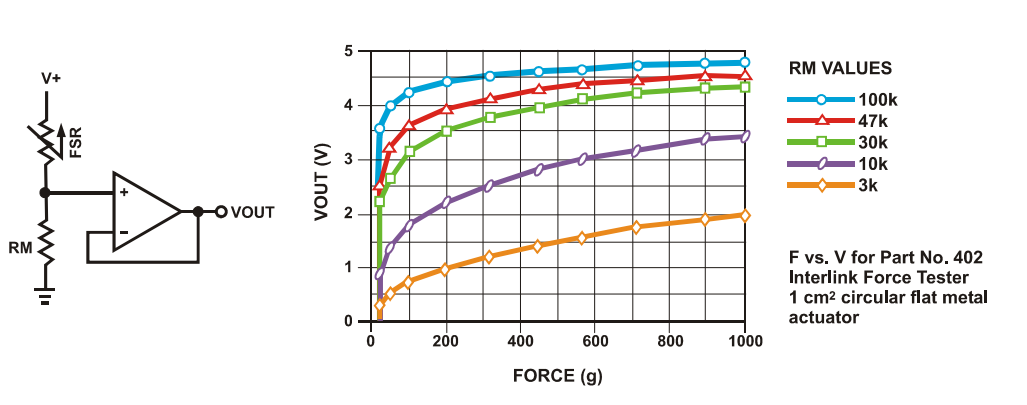
\includegraphics[width=\textwidth]{Figure/fsr.png}
\caption{FSR Voltage Divider}
\label{Fig:FSRcircuit}
\end{figure}


 The physical position of the FSR sensors is shown in the figure \ref{fig:sensors}
\begin{figure}[!tbp]
  \centering
  \begin{minipage}[b]{0.4\textwidth}
    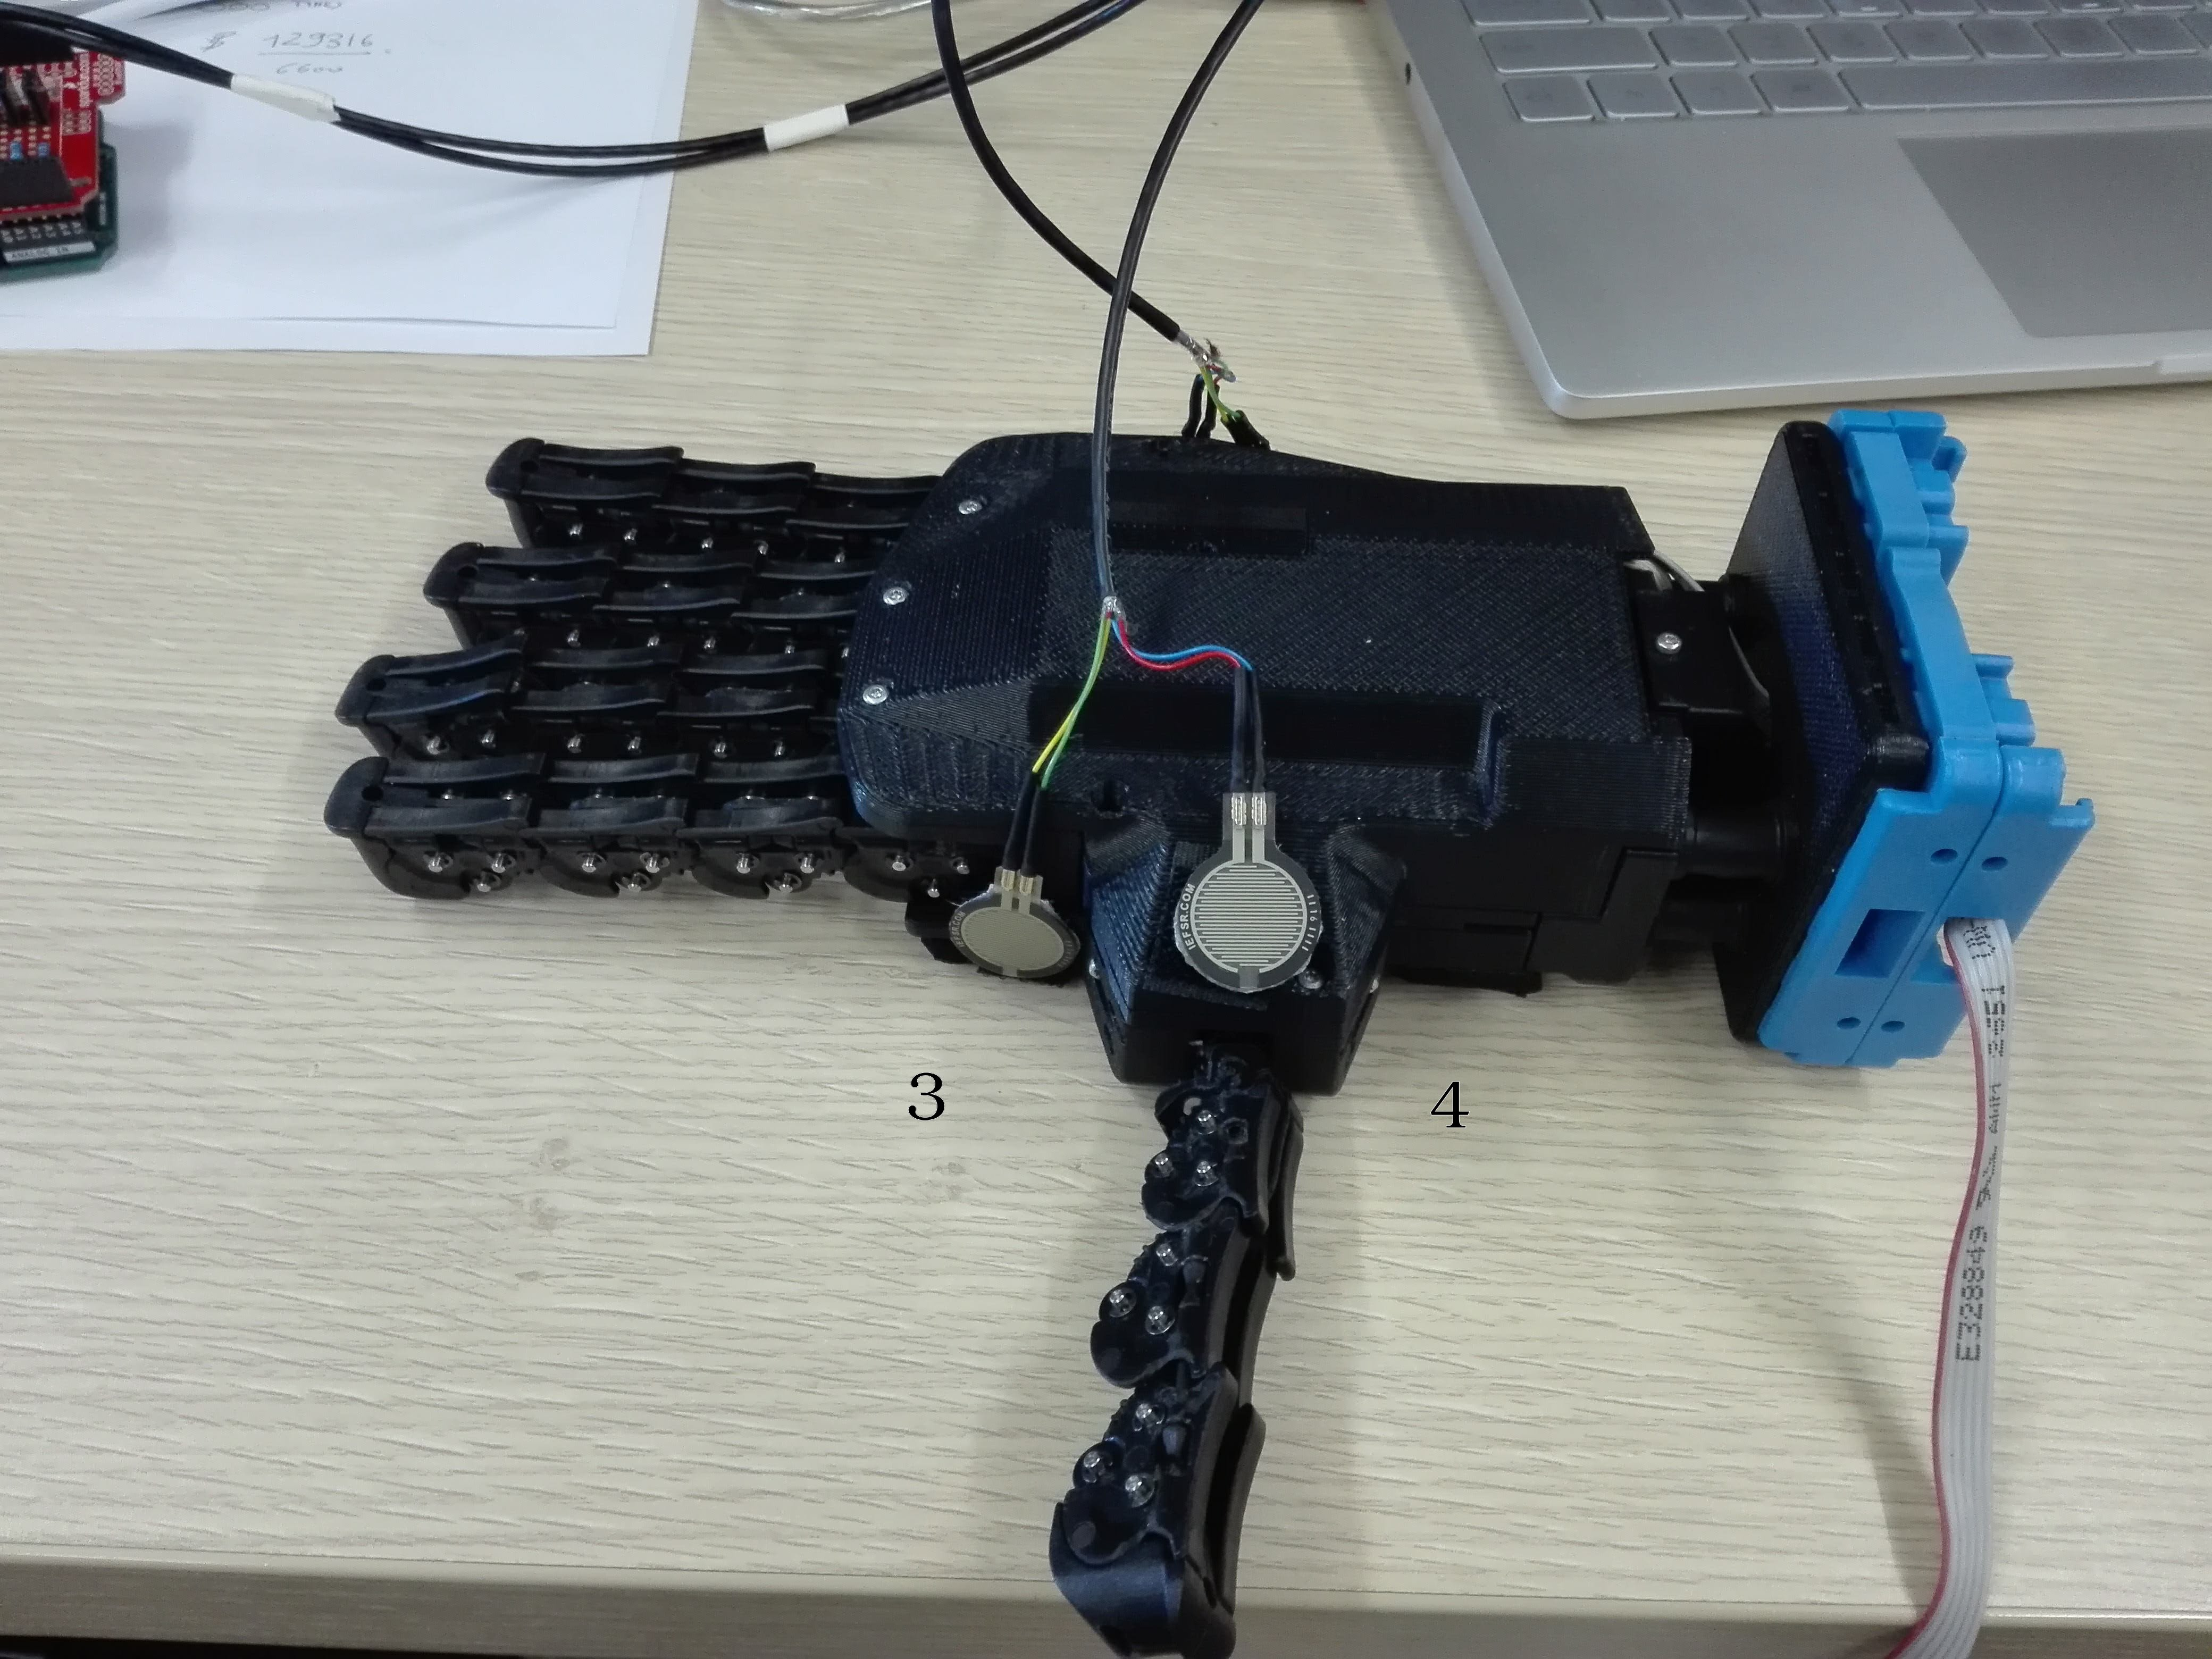
\includegraphics[width=\textwidth]{Figure/qbhand1.jpg}
    
  \end{minipage}
  \hfill
  \begin{minipage}[b]{0.4\textwidth}
    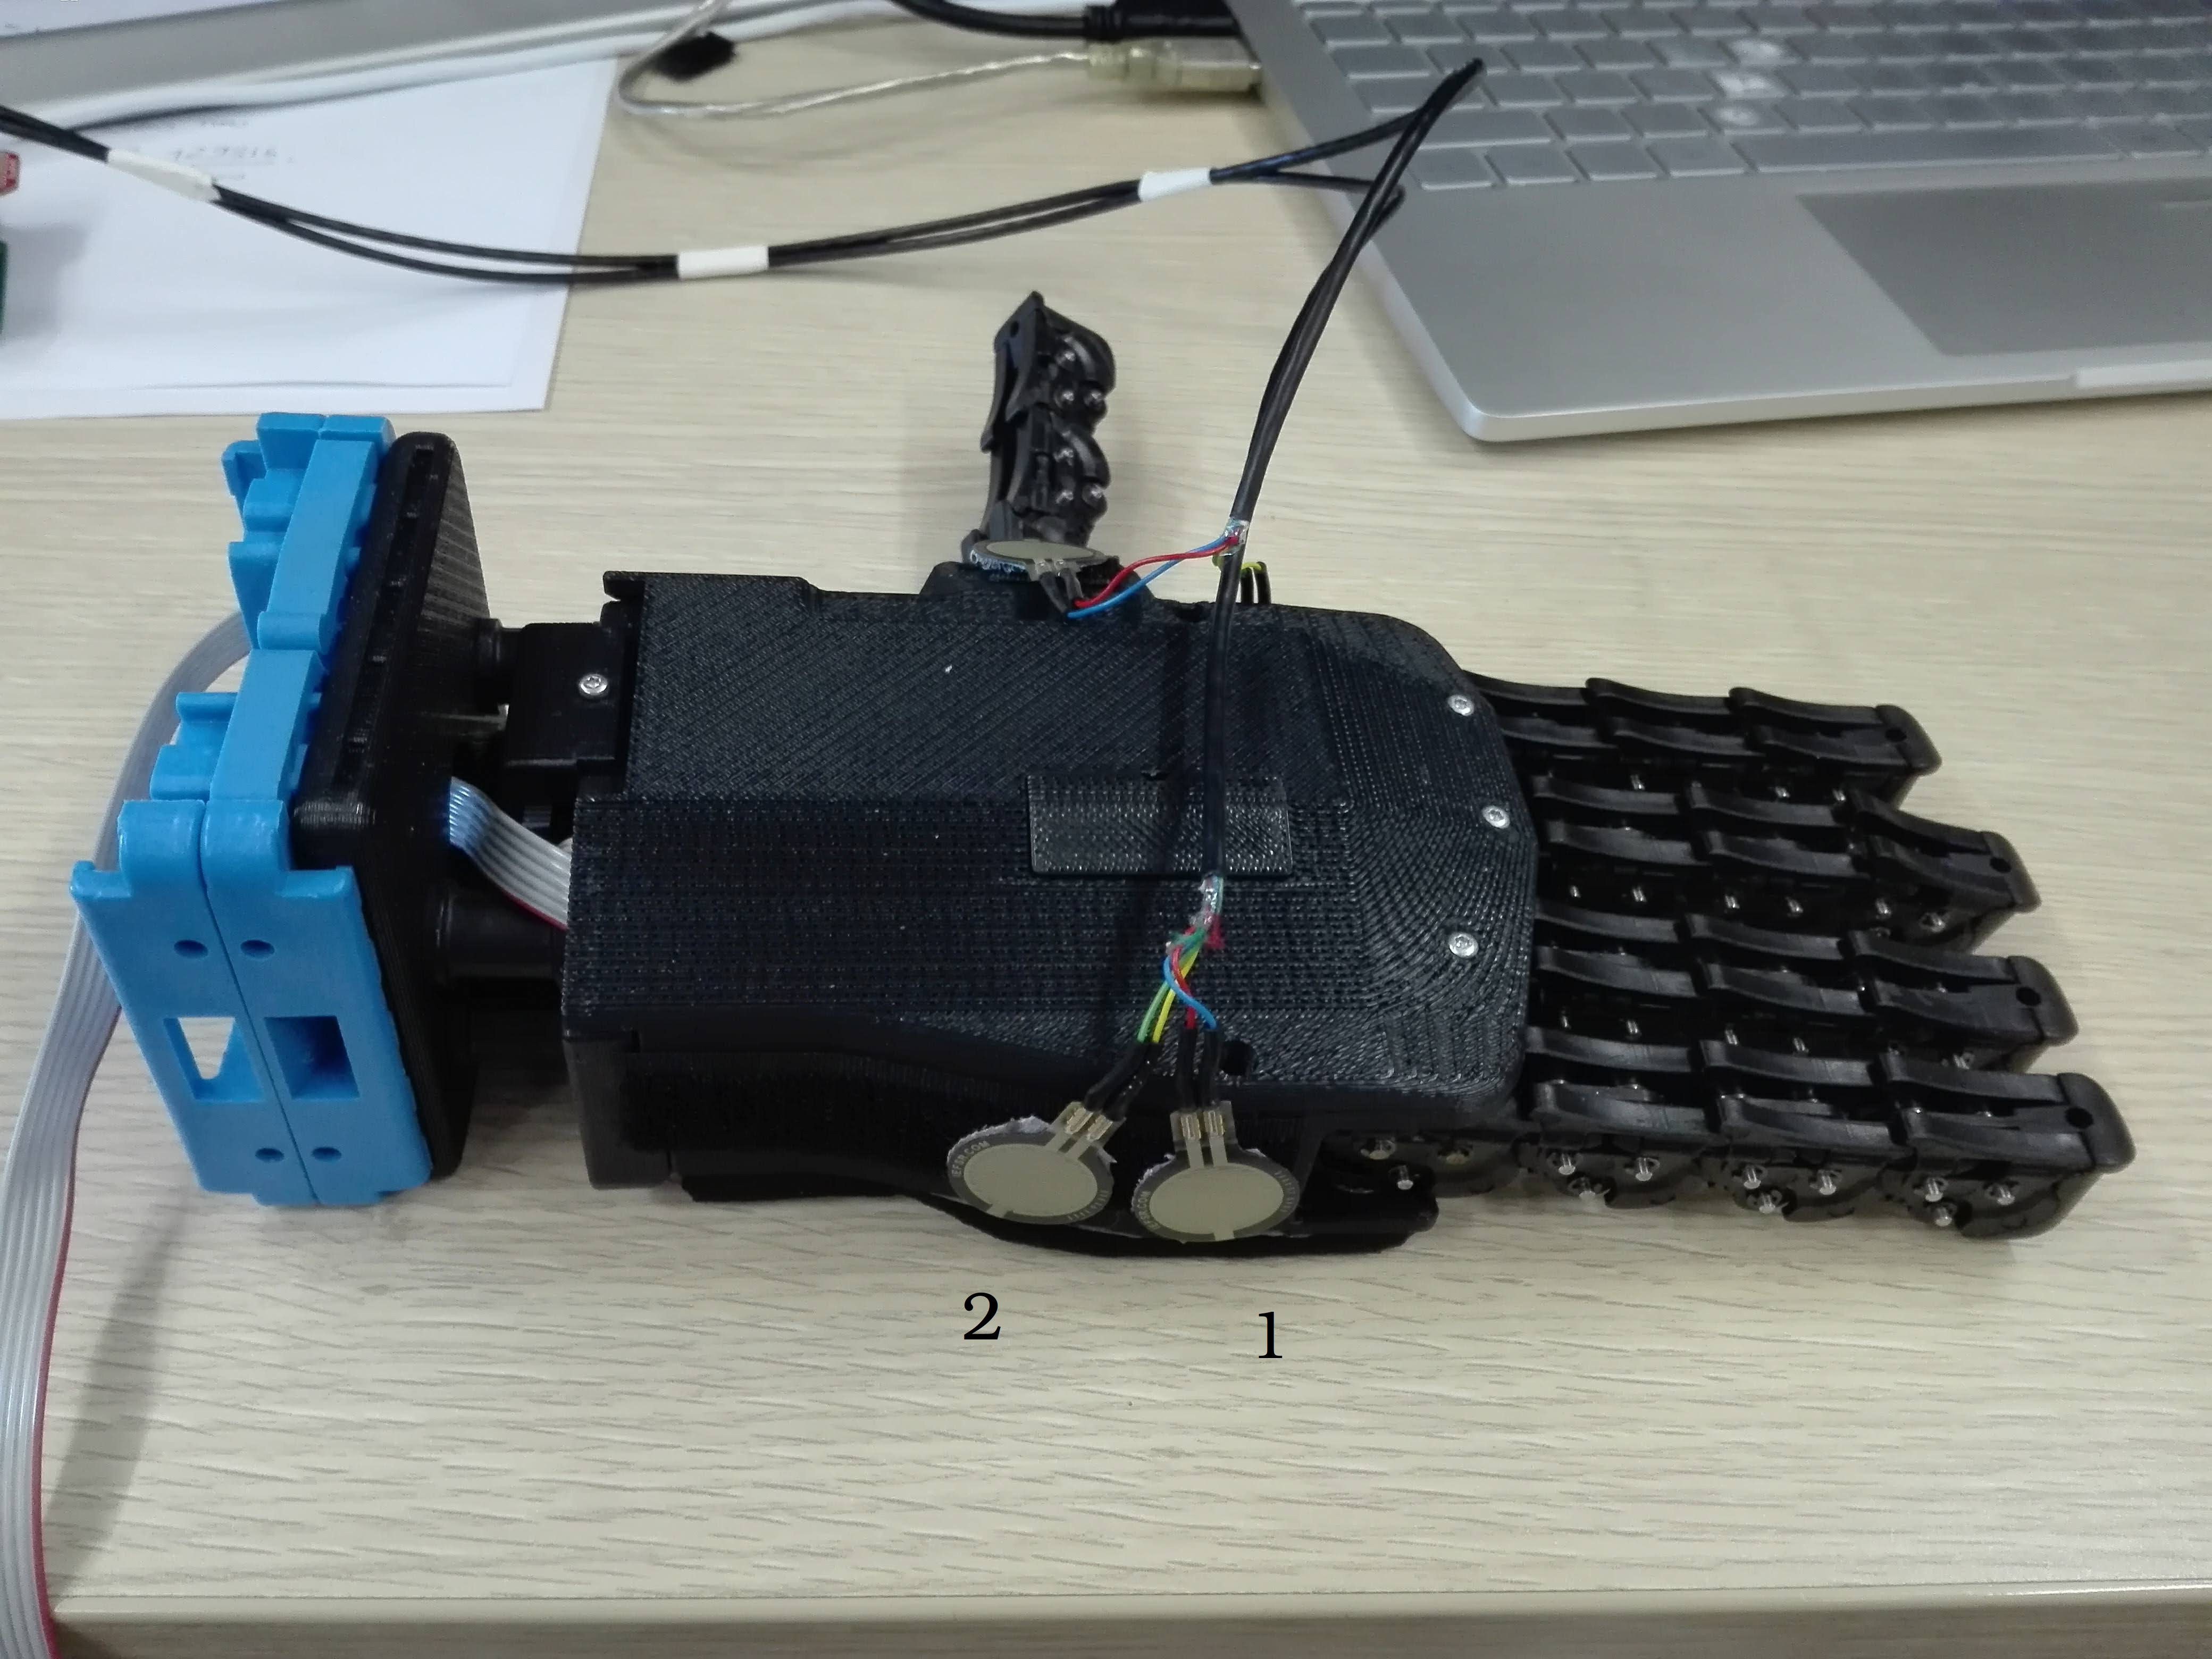
\includegraphics[width=\textwidth]{Figure/qbhand2.jpg}
  \end{minipage}
  \label{fig:sensors}
  \caption{FSR sensors position}
\end{figure}

\section{}
\chapter{Software setup}
\section{Ros}


\chapter*{Conclusion}
This project applies learning \cite{art:rif.1} techniques to MNIST handwritten dataset. As we can see in the previous confusion matrix the accuracy of the final work is $97.6\%$. The overall idea is to train \emph{autoenc1},  \emph{autoenc2} and \emph{softmax1} once per time and to crop the nets in order to have coherents dimension between network interconnections. At the end of \cite{book:rif.2}this process we stack all the partial neural network together and the deep neural network come to life. \\The satisfaction behind this project can be experimented by running the file "MNIST\textunderscore drawsim.m" which is a matlab function that allows the user to draw a digit and returns the correct digit value 97,6 times over 100.